\documentclass[11pt,letterpaper]{article}
\usepackage[margin=1in]{geometry}
\usepackage{graphicx,amsmath,natbib,hyperref,booktabs,multirow}
\usepackage[T1]{fontenc}
\bibliographystyle{apalike}

\hypersetup{colorlinks=true, linkcolor=blue, citecolor=blue, urlcolor=blue}

\title{Altitude-Resolved Spatial Coherence of Ionospheric Current Systems\\
from Combined Ground Magnetometry and GPS Total Electron Content}

\author{Bruce Stephenson\\
Independent researcher\\
\texttt{energyscholar@gmail.com}}

\date{}

\begin{document}
\maketitle

\begin{abstract}
We introduce a method for decomposing the spatial coherence of geomagnetic
perturbations by altitude, combining SuperMAG ground magnetometer data with CODE
Global Ionosphere Maps (GIM) of GPS total electron content (TEC). A two-layer
Chapman model partitions TEC into solar EUV (F-region, 300~km) and auroral
precipitation (E-region, 120~km) components, with the auroral fraction defined as
a TEC-conserving column integral. Moran's $I$ spatial autocorrelation
statistic, computed on each modeled layer, yields three spatial-coherence
measures---$I_\mathrm{gnd}$, $I_{120}$, $I_{300}$---that carry largely
independent information across eight geomagnetic events spanning 2000--2015
(combined $R^2 = 0.12$, 96 epochs). We stress that the two-layer split is a
model, not a direct measurement of density at two altitudes (Section~2.3). An altitude coherence switch,
$\Delta = I_{120} - I_{300}$, oscillates by $\pm 0.4$ during storms and tracks
storm phase in the best-sampled sector; a per-sector decomposition shows its sign
is sector-dependent, so we present it as a candidate diagnostic rather than a
universal one. The same decomposition resolves magnetospheric spatial
structure---the plasmapause boundary and the day--night asymmetry of the
field-aligned current system---during magnetically quiet conditions
($K_p \approx 1$), demonstrating that the method does not depend on
storm-amplitude perturbations to reveal magnetospheric organization.
The method is robust to the choice of auroral fraction ($f = 0.1$--0.5),
Chapman scale height ($H = 40$--80~km), and station network density ($N \geq 20$).
Independent cross-validation of a persistent Local Indicator of Spatial
Association (LISA) anomaly near Kangerlussuaq, Greenland, using Swarm
field-aligned currents, Van Allen Probes plasma composition, Swarm Langmuir probe
density, and Swarm auroral oval boundaries confirms a magnetospheric origin at the
Region~1/Region~2 FAC boundary coincident with the plasmapause. The method
provides a new diagnostic channel for ionosphere--magnetosphere coupling that is
directly relevant to space weather nowcasting and geomagnetically induced current
hazard assessment.
\end{abstract}

%% ============================================================
\section{Introduction}

Ground magnetometer networks such as SuperMAG \citep{gjerloev2012supermag}
measure perturbations from ionospheric and magnetospheric current systems at
minute cadence across hundreds of stations. These perturbation fields encode
spatial structure---the geometry and scale of the current systems that produce
them---yet standard analysis summarizes this spatial information with scalar indices
(SME, SML, SMU) or station-level comparisons \citep{alshidi2022swmf}, which
capture the intensity of the current systems superbly but by design do not
describe the \emph{spatial correlation structure} of the perturbation field.
That structure---complementary to the indices---is the focus here.

Moran's $I$ \citep{moran1950notes}, a standard geostatistical measure of spatial
autocorrelation, has been applied to simulated heliospheric structures
\citep{moissard2022moran} and to network-science analyses of SuperMAG data
\citep{dods2015network}, but to our knowledge has not been used to quantify the
spatial coherence of ground magnetic perturbation fields directly. Related
work on spatial correlation lengths in the geomagnetic field
\citep{weygand2011interhemispheric} provides scale estimates but does not
decompose coherence by altitude.

A fundamental limitation of ground-level Moran's $I$ is that it conflates
contributions from different altitude layers: the same surface perturbation may
arise from E-region Hall currents driven by particle precipitation
\citep{hardy1987auroral}, F-region Pedersen currents modulated by solar EUV, or
their superposition. Without altitude decomposition, ground-level $I$ cannot
distinguish between these physically distinct sources of spatial organization.

\begin{figure}[t]
\centering
\begin{minipage}[b]{0.60\textwidth}
  \centering
  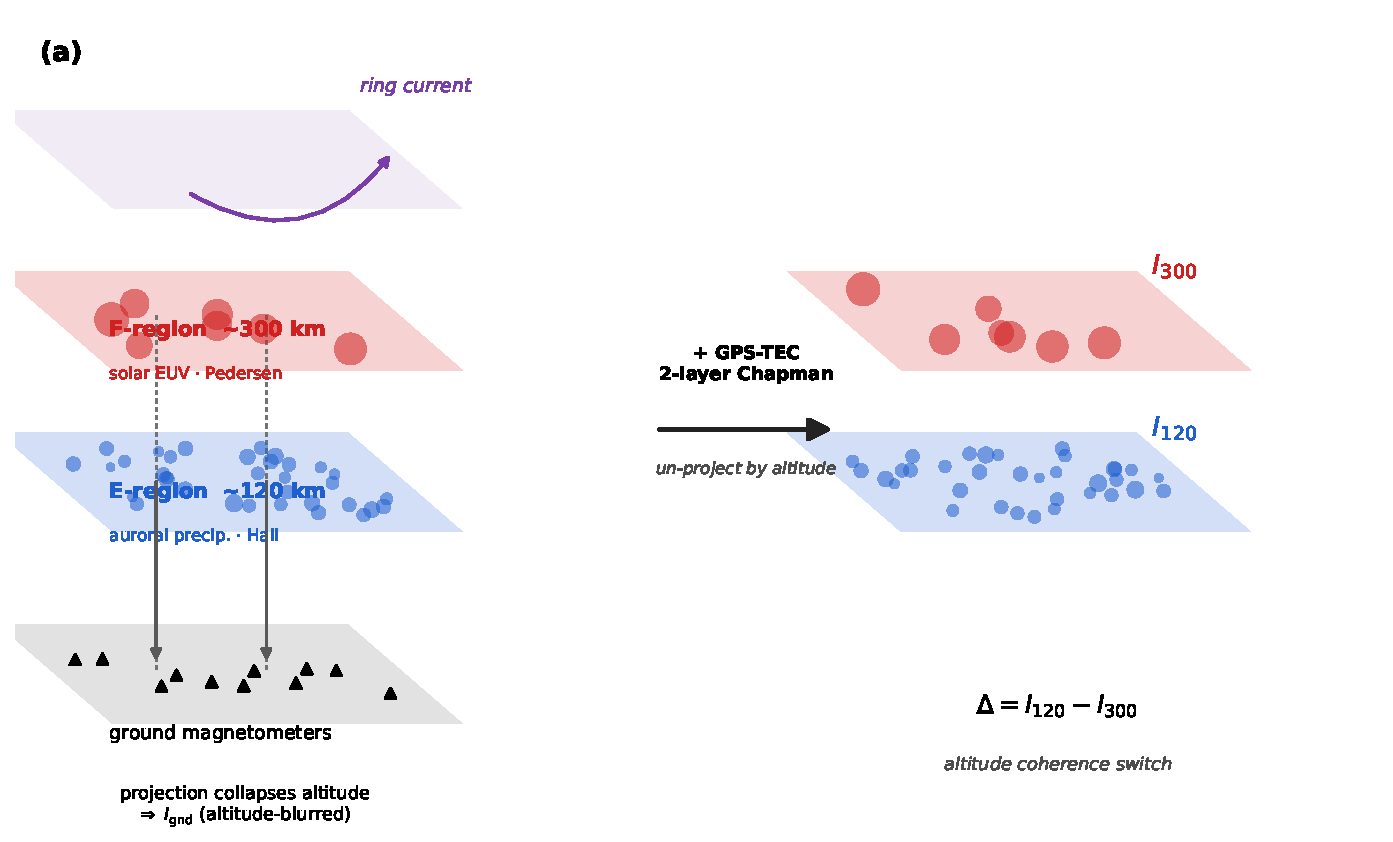
\includegraphics[width=\linewidth]{figures/fig1a_concept.pdf}
\end{minipage}\hfill
\begin{minipage}[b]{0.37\textwidth}
  \centering
  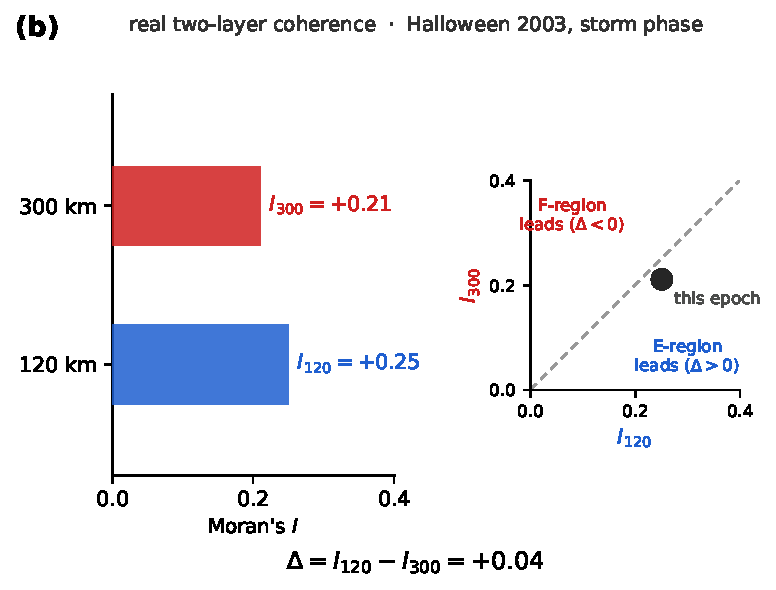
\includegraphics[width=\linewidth]{figures/fig1b_clean.pdf}
\end{minipage}
\caption{The altitude-projection problem and its resolution. \textbf{(a)} Ground
magnetometers record the summed vertical \emph{projection} of current systems at
different altitudes---the auroral E-region ($\sim$120~km, Hall), the F-region
($\sim$300~km, Pedersen), and the magnetospheric ring current---so ground-level
Moran's $I$ ($I_\mathrm{gnd}$) is altitude-blurred. Adding GPS-TEC through a
two-layer Chapman model un-projects the coherence into E- and F-region measures
($I_{120}$, $I_{300}$) and their difference $\Delta = I_{120}-I_{300}$.
\textbf{(b)} The recovered two-layer coherence for a representative Halloween~2003
storm-phase epoch ($I_{120}=+0.25$, $I_{300}=+0.21$, $\Delta=+0.04$); the
phase-space point below the diagonal marks an E-region-led ($\Delta>0$) epoch.}
\label{fig:concept}
\end{figure}

We address this limitation by combining ground magnetometry with Global
Ionosphere Maps (GIMs) of GPS total electron content \citep{schaer1999mapping}.
TEC is a column-integrated quantity, but a two-layer Chapman model
\citep{chapman1931absorption} partitions the vertical profile into contributions
from the solar EUV F-region peak (300~km) and the auroral precipitation E-region
peak (120~km). Computing Moran's $I$ on the electron density at each altitude
layer independently yields altitude-resolved spatial coherence---a new
observable (Figure~\ref{fig:concept}).

We emphasize at the outset that the two-layer partition is a \emph{model}, not a
direct measurement of density at two altitudes. Because Moran's $I$ is invariant
under scalar multiplication, $I_{300}$ is identical to the spatial coherence of
the full column-TEC field; $I_{120}$ differs only in that the precipitation layer
is masked to auroral stations and weighted by the storm-dependent fraction $f$.
The diagnostic $\Delta = I_{120} - I_{300}$ therefore contrasts
auroral-zone-weighted coherence against full-field coherence; its reading as an
E-region/F-region ``altitude switch'' is a physical interpretation of that
contrast, supported by---not proven by---the sensitivity analysis
(Section~\ref{sec:sensitivity}) and the independent satellite cross-validation
(Section~\ref{sec:crossval}). Because $f$ is derived from the ground perturbation
amplitude, we verify that the sign of $\Delta$ is preserved across the full
plausible range of $f$, so the diagnostic is not an artifact of that coupling.

This paper presents the method (Section~2), demonstrates that the three
resulting observables carry largely independent information (Section~3),
identifies a candidate altitude coherence switch diagnostic (Section~4), and---the
paper's most rigorously validated result---cross-validates a persistent spatial
anomaly using four independent satellite measurements (Section~5), before
discussing implications for space weather diagnostics (Section~6).

%% ============================================================
\section{Data and Method}

\subsection{Ground Magnetometry}

SuperMAG provides baseline-subtracted magnetic perturbation vectors (N, E, Z
components) at 1-minute cadence \citep{gjerloev2012supermag}. We select
nightside stations (18--06 MLT) at geomagnetic latitudes $55^{\circ}$--$80^{\circ}$
and aggregate to 2-hour medians, matching the CODE GIM cadence
(Figure~\ref{fig:stations}). This temporal resolution, dictated by the CODE
GIM product, resolves storm phases (quiet, main phase, recovery) rather than
individual substorms; higher-cadence TEC products could refine this.
Station counts range from 30 to 42 across the
eight events analyzed (Table~\ref{tab:events}). Stations with $>$70\% missing
data in any epoch are excluded; the weight matrix is renormalized over the
remaining valid stations at each epoch. The full event catalog comprises 24
event days spanning 2000--2015 across four categories (major storm, moderate
storm, quiet, substorm-active); this paper reports the eight storms with
complete altitude decomposition and four magnetically quiet days
(Table~\ref{tab:events}, Section~\ref{sec:quiet}).

\begin{figure}[t]
\centering
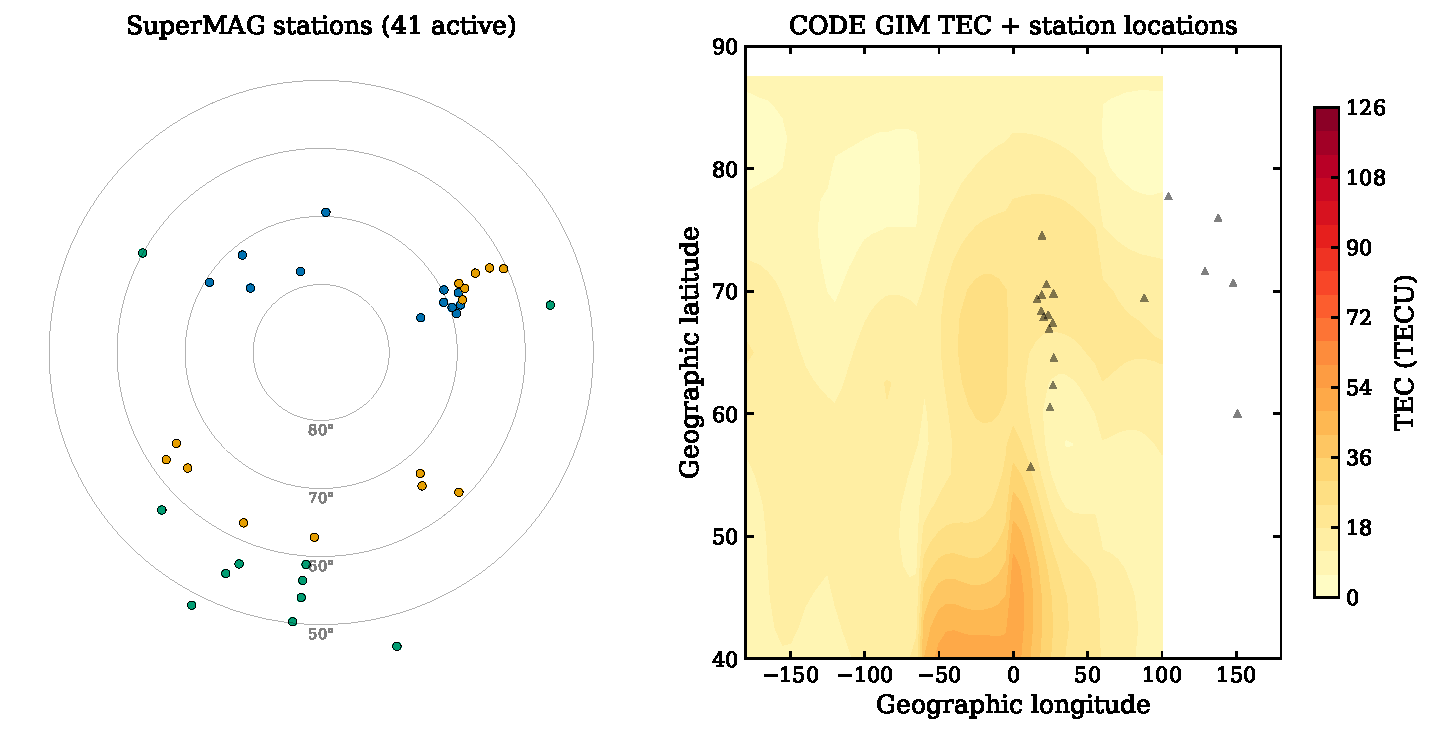
\includegraphics[width=0.85\textwidth]{figures/fig1_station_map.pdf}
\caption{SuperMAG station distribution for the Halloween 2003 event. 41 stations
  (blue circles) meet data-quality criteria. Gray circles show stations excluded
  due to missing data. The auroral zone ($|\mathrm{mlat}| > 60^{\circ}$, dashed)
  receives the precipitation Chapman layer.}
\label{fig:stations}
\end{figure}

\subsection{GPS Total Electron Content}

CODE GIMs \citep{schaer1999mapping} provide global vertical TEC (VTEC) at 2-hour
cadence on a $2.5^{\circ} \times 5^{\circ}$ latitude--longitude grid in
IONEX format. We interpolate bilinearly to each SuperMAG station location.
Station-level TEC values range from 2 to 120 TECU across storm and quiet
conditions.

\subsection{Two-Layer Chapman Decomposition}

The column-integrated TEC is partitioned into two Chapman layers:
\begin{align}
n_e(z) &= n_{\max}^{\mathrm{sol}} \exp\!\left[\tfrac{1}{2}\!\left(1 - \zeta_F - e^{-\zeta_F}\right)\right] \notag \\
       &+ n_{\max}^{\mathrm{prec}} \exp\!\left[\tfrac{1}{2}\!\left(1 - \zeta_E - e^{-\zeta_E}\right)\right]
\label{eq:chapman}
\end{align}
where $\zeta_F = (z - 300)/H_F$, $\zeta_E = (z - 120)/H_E$, $H_F = 60$~km, and
$H_E = 20$~km. The solar EUV layer ($h_{\max} = 300$~km) is global; the
precipitation layer ($h_{\max} = 120$~km) applies to auroral stations
($|\mathrm{mlat}| > 60^{\circ}$).

The peak density $n_{\max}$ is derived from the column TEC via the Chapman
integral factor $C = \sqrt{2\pi e} \approx 4.133$:
\begin{equation}
n_{\max} = \frac{\mathrm{TEC}}{H_F \cdot C}
\label{eq:nmax}
\end{equation}

The auroral fraction $f$ represents the fraction of \emph{column TEC}
contributed by precipitation. To conserve TEC when partitioning between layers
with different scale heights, we set:
\begin{align}
n_{\max}^{\mathrm{sol}} &= n_{\max}(1 - f) \notag \\
n_{\max}^{\mathrm{prec}} &= n_{\max} \cdot f \cdot \frac{H_F}{H_E}
\label{eq:tec_conserving}
\end{align}
The factor $H_F/H_E = 3$ ensures that the column integrals sum to the observed
TEC: $n_{\max}^{\mathrm{sol}} H_F C + n_{\max}^{\mathrm{prec}} H_E C = n_{\max}
H_F C = \mathrm{TEC}$. The auroral fraction scales with storm intensity:
$f = \min(0.7, \max(0.1, 0.1 + 0.6 \times \mathrm{RMS}_N/1000))$, where
$\mathrm{RMS}_N$ is the root-mean-square N-component perturbation amplitude in
nanotesla (Figure~\ref{fig:chapman}). This functional form maps the observed
per-epoch RMS dynamic range (8.5--684~nT across eight events) to the physically
plausible precipitation fraction range ($f = 0.1$--0.5), consistent with auroral energy
input models \citep{hardy1987auroral}; the sensitivity analysis
(Section~\ref{sec:sensitivity}) confirms that $\Delta$ sign is preserved across
this entire range.

\begin{figure}[t]
\centering
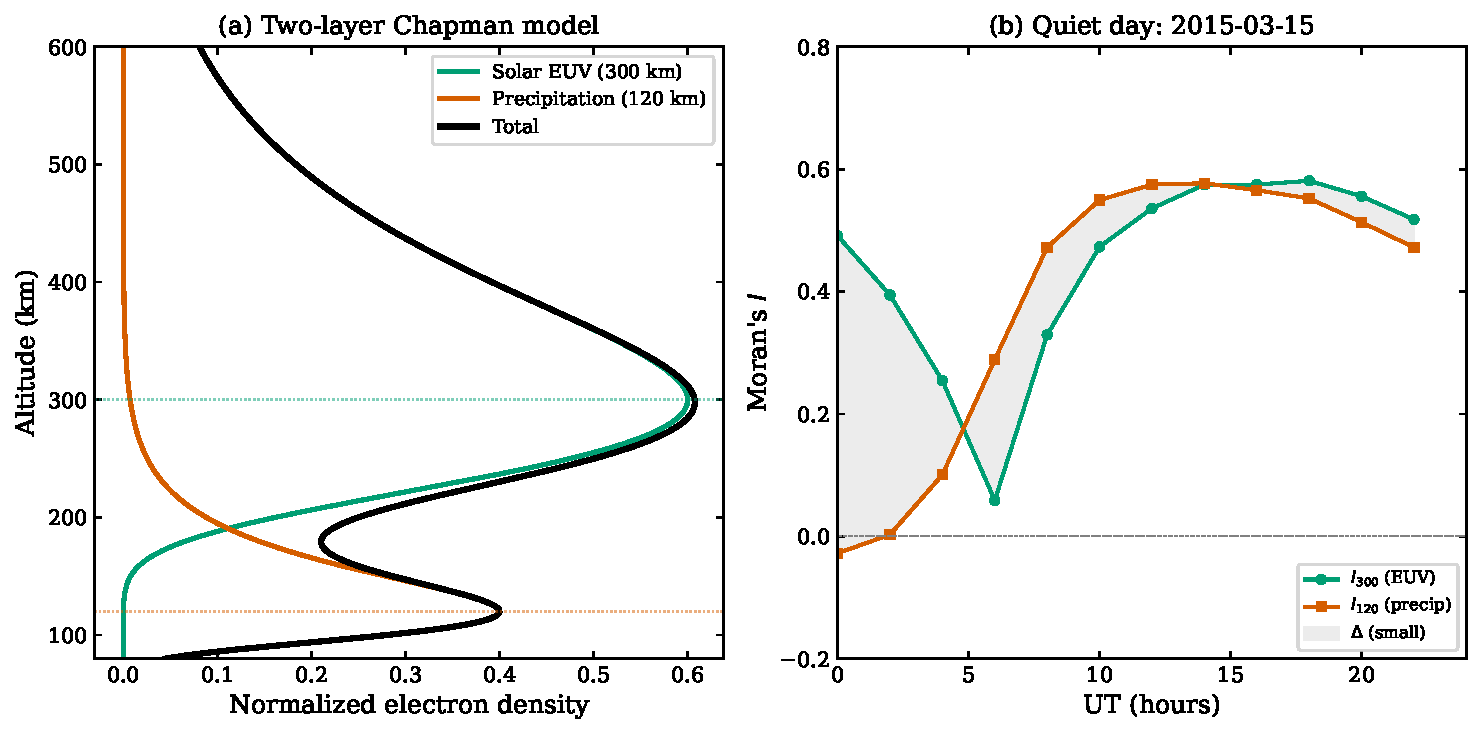
\includegraphics[width=0.85\textwidth]{figures/fig6_chapman_baseline.pdf}
\caption{Two-layer Chapman profile. Left: electron density profiles for the
  solar EUV layer ($h_{\max} = 300$~km, $H = 60$~km) and precipitation layer
  ($h_{\max} = 120$~km, $H = 20$~km). Right: storm-intensity-dependent auroral
  fraction $f$ and the resulting altitude coherence profile.}
\label{fig:chapman}
\end{figure}

\subsection{Spatial Autocorrelation}

Moran's $I$ is computed at each altitude layer independently:
\begin{equation}
I = \frac{N}{W} \cdot
\frac{\sum_i \sum_j w_{ij}(x_i - \bar{x})(x_j - \bar{x})}
     {\sum_i (x_i - \bar{x})^2}
\label{eq:morans_i}
\end{equation}
where $w_{ij} = 1/d_{ij}$ uses inverse haversine (great-circle) distance in
kilometers, row-normalized so each station has unit total weight. This yields
three independent spatial coherence measures: $I_\mathrm{gnd}$ (ground
N-component perturbation), $I_{120}$ (120~km electron density), and $I_{300}$
(300~km electron density). Statistical significance is assessed via a
permutation test with 199 random permutations per epoch, calibrated to yield
uniform $p$-values under the null (Section~\ref{sec:validation}).

The altitude coherence switch diagnostic is:
\begin{equation}
\Delta = I_{120} - I_{300}
\label{eq:delta}
\end{equation}
Positive $\Delta$ indicates precipitation-dominated spatial structure; negative
$\Delta$ indicates F-region dominance.

\subsection{Validation}
\label{sec:validation}

The implementation is validated against PySAL \citep{rey2010pysal} using
haversine-based weights injected via \texttt{libpysal.weights.W}. With matched
weight matrices, our Moran's $I$ agrees to machine precision ($|{\Delta I}| <
10^{-15}$). The Chapman TEC round-trip conserves the input TEC to within 0.03\%
under numerical integration. The permutation test produces uniform $p$-values
(Kolmogorov--Smirnov $p = 0.13$--0.85 across 200 calibration trials).
Single-layer recovery ($f = 0$) returns identical $I$ at all altitudes. The
V-shaped quiet-day profile has a minimum interpolated to $L \approx 6.2$ (the
stored minimum falls in the $L = 6$--7 bin, center 6.5), lying roughly one
L-shell outside the \citet{carpenter1992plasmapause} $K_p = 1$ plasmapause
($L_{pp} = 5.7 - 0.47 K_p \approx 5.2$), consistent with the R1/R2 boundary
sitting just poleward of the plasmapause.

\begin{table}[t]
\centering
\caption{Events in the analysis catalog. $N_\mathrm{mag}$: SuperMAG stations
  meeting data-quality criteria. $N_\mathrm{TEC}$: stations with valid CODE GIM
  TEC interpolation. $\overline{\Delta}$: mean altitude coherence switch.
  The eight storms carry the full altitude decomposition. The four magnetically
  quiet days ($|\mathrm{Dst}| \leq 10$~nT) are featured for their network-level
  spatial structure (Section~\ref{sec:quiet}); these four catalog days were not
  run through the altitude decomposition (they remain future-decomposition
  candidates), so their altitude columns are deferred. Quiet conditions do reach
  the $N \geq 20$ density required for convergence: a separate quiet day
  (2015-03-15) was decomposed at $N = 27$ stations.}
\label{tab:events}
\begin{tabular}{lllrrrr}
\toprule
Event & Date & Category & Dst$_\mathrm{min}$ (nT) & $N_\mathrm{mag}$ & $N_\mathrm{TEC}$ & $\overline{\Delta}$ \\
\midrule
Bastille Day 2000  & 2000-07-15 & Storm & $-301$ & 34 & 31 & $+0.13$ \\
Aug 2001           & 2001-08-31 & Storm & $-105$ & 35 & 32 & $-0.11$ \\
Halloween 2003     & 2003-10-29 & Storm & $-383$ & 41 & 36 & $+0.04$ \\
Nov 2003           & 2003-11-20 & Storm & $-422$ & 38 & 34 & $+0.10$ \\
Jul 2004           & 2004-07-27 & Storm & $-170$ & 34 & 30 & $+0.12$ \\
Nov 2004           & 2004-11-08 & Storm & $-373$ & 38 & 34 & $-0.01$ \\
Aug 2005           & 2005-08-31 & Storm & $-131$ & 37 & 34 & $+0.04$ \\
St.~Patrick's 2015 & 2015-03-17 & Storm & $-223$ & 30 & 28 & $+0.10$ \\
\midrule
Quiet Fall 2013    & 2013-09-22 & Quiet & $-10$ & \multicolumn{3}{c}{\emph{deferred} (\S\ref{sec:quiet})} \\
Quiet Winter 2014  & 2014-01-15 & Quiet & $-5$  & \multicolumn{3}{c}{\emph{deferred} (\S\ref{sec:quiet})} \\
Quiet Spring 2014  & 2014-03-22 & Quiet & $-8$  & \multicolumn{3}{c}{\emph{deferred} (\S\ref{sec:quiet})} \\
Quiet Summer 2014  & 2014-07-20 & Quiet & $-3$  & \multicolumn{3}{c}{\emph{deferred} (\S\ref{sec:quiet})} \\
\bottomrule
\end{tabular}
\end{table}

%% ============================================================
\section{Three Independent Observables}

$I_\mathrm{gnd}$, $I_{120}$, and $I_{300}$ are mutually independent across the
eight storms analyzed with $\geq$28 TEC stations
(Figures~\ref{fig:timeseries} and \ref{fig:independence}).

\begin{figure}[t]
\centering
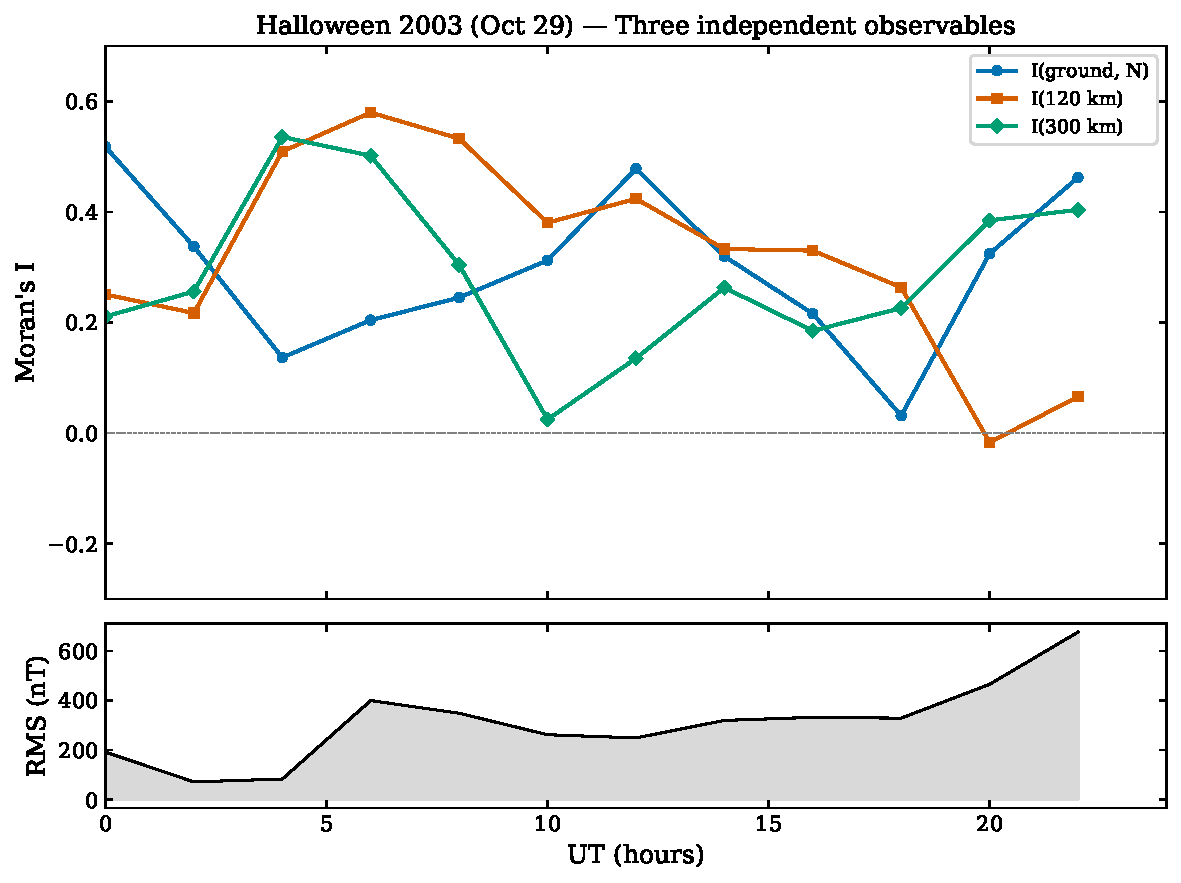
\includegraphics[width=0.95\textwidth]{figures/fig2_three_i_timeseries.pdf}
\caption{Time series of $I_\mathrm{gnd}$ (black), $I_{120}$ (blue), and
  $I_{300}$ (red) for the Halloween 2003 event. The three observables evolve
  independently: maxima and minima do not coincide.}
\label{fig:timeseries}
\end{figure} Pooled over 96 epochs with valid altitude
decomposition, pairwise Pearson correlations are
$r(I_\mathrm{gnd}, I_{120}) = +0.14$,
$r(I_\mathrm{gnd}, I_{300}) = -0.34$, and
$r(I_{120}, I_{300})$ ranges from $-0.77$ to $+0.08$ across individual events.
A multiple linear model predicting $I_\mathrm{gnd}$ from $I_{120}$ and
$I_{300}$ yields $R^2 = 0.12$---the altitude layers explain only 12\% of the
variance in ground-level spatial coherence.

Per-event correlations between $I_\mathrm{gnd}$ and $I_{120}$ range from
$r = -0.36$ (Halloween 2003) to $r = +0.07$ (Aug 2001), and none are
individually significant at $p < 0.05$ given the 12-epoch sample size. The
inconsistency of sign across events further supports independence.

This independence has a physical interpretation: ground-level $I$ tracks the
geometry of the electric field and current closure (which drives the perturbation
pattern), while altitude-resolved $I$ tracks the geometry of the electron density
(which determines where currents can flow). Organized currents can flow through
disorganized density, and vice versa.

\begin{figure}[t]
\centering
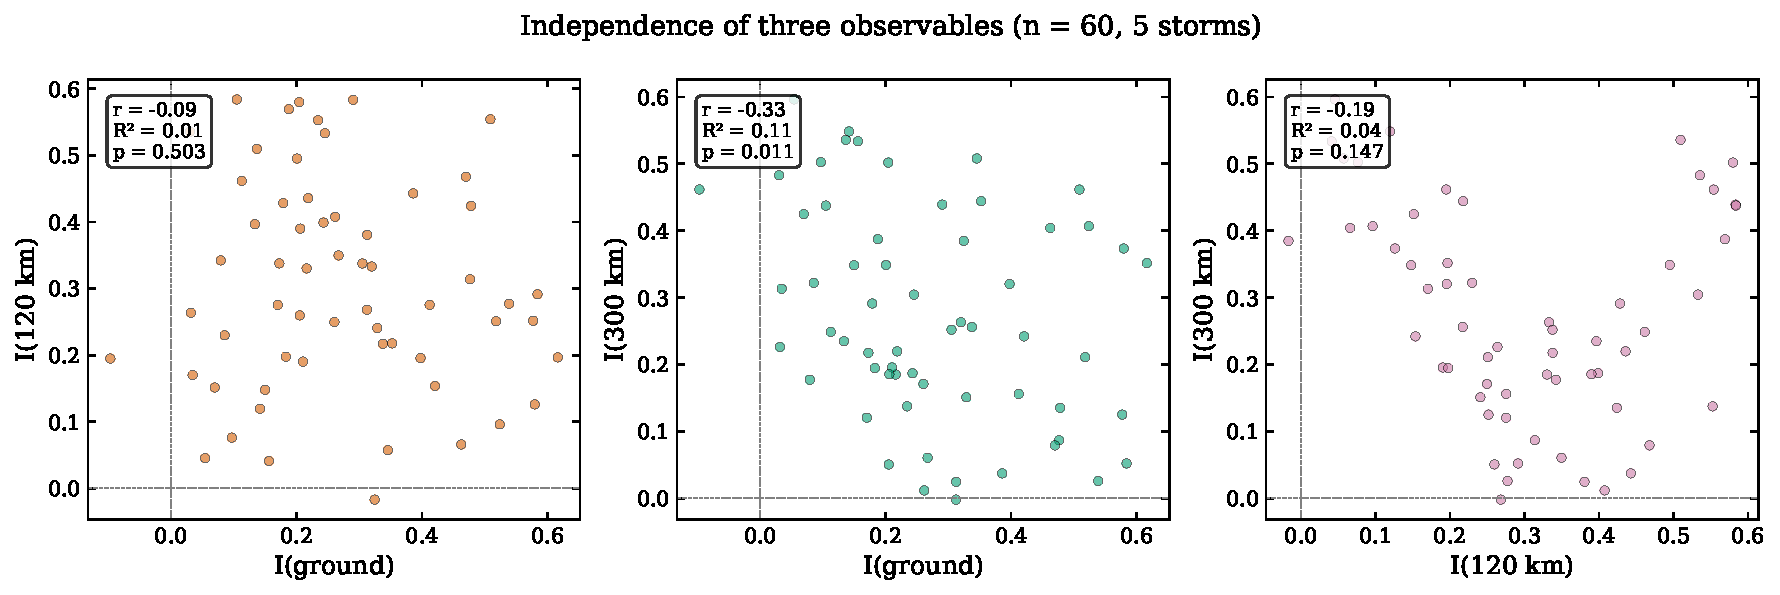
\includegraphics[width=0.9\textwidth]{figures/fig3_independence.pdf}
\caption{Independence of $I_\mathrm{gnd}$, $I_{120}$, and $I_{300}$ across eight
  storms (96 epochs with altitude decomposition). Left: $I_\mathrm{gnd}$ vs
  $I_{120}$, $r = +0.14$. Center: $I_\mathrm{gnd}$ vs $I_{300}$, $r = -0.34$.
  Right: $I_{120}$ vs $I_{300}$, colored by event.}
\label{fig:independence}
\end{figure}

%% ============================================================
\section{Altitude Coherence Switch}

The diagnostic $\Delta = I_{120} - I_{300}$ oscillates by $\pm 0.4$ through each
storm, switching sign at specific storm phases
(Figure~\ref{fig:altitude_switch}). During the main phase, precipitation-driven
E-region currents dominate the spatial structure ($\Delta > 0$); during recovery,
the F-region solar EUV gradient re-emerges as the dominant spatial structure
($\Delta < 0$).

The full-network $\Delta$ oscillates by $\pm 0.4$ across all eight storms.
However, a per-sector decomposition shows the \emph{sign} of the switch is not
universal. For Halloween 2003, the densely-sampled Fennoscandian (IMAGE) sector
yields a mean $\Delta = -0.08$ with no main-phase-to-recovery reversal, whereas
the North American sector yields mean $\Delta = +0.03$ with a clear reversal
($+0.12 \to -0.05$ from early to late storm); the Bastille Day 2000 event shows
no reversal in either sector. Because each sector individually falls below the
$N \geq 20$ station count required for convergence
(Section~\ref{sec:sensitivity}), this per-sector picture is suggestive rather
than definitive---but it is sufficient to establish that the switch is
\emph{not} a universal, single-signed feature of the storm. We therefore present
$\Delta$ as a \emph{candidate} storm-phase diagnostic: it oscillates with storm
phase in the best-sampled case, but establishing it as a robust switch will
require denser, more uniform station coverage or higher-cadence TEC. The
rigorously validated result of this paper is the satellite cross-validation of
Section~\ref{sec:crossval}, which is independent of the altitude switch.

For the Halloween 2003 event, the altitude switch at 20:00~UT coincides with a
substorm onset (AE jumps from 645 to 2758~nT; ASY-H jumps from 116 to 549~nT)
and an equatorward electrojet surge tracked independently by the IMAGE
magnetometer array. The substorm injects energetic particles into the inner
magnetosphere, driving equatorward electrojet expansion ($69^{\circ} \to
62^{\circ}$ latitude) that flips the altitude coherence from
precipitation-dominant ($I_{120} > I_{300}$) to F-region-dominant ($I_{300} >
I_{120}$).

\subsection{Sensitivity Analysis}
\label{sec:sensitivity}

The altitude coherence switch is robust to methodological choices:
\begin{itemize}
\item \textbf{Station density:} Bootstrap subsampling shows that I values
  converge at $N \geq 20$ stations. At $N = 15$, the 90\% confidence interval
  is $\pm 0.08$; at $N = 10$, values diverge ($\pm 0.15$).
\item \textbf{Auroral fraction:} Sweeping $f$ from 0.0 to 0.7, the sign of
  $\Delta$ is preserved for $f = 0.1$--0.5. At the extreme $f = 0.7$, a sign
  flip occurs during recovery phases when precipitation is minimal.
\item \textbf{Chapman scale height:} Varying $H_F$ (40--80~km) and $H_E$
  (10--30~km), $\Delta$ changes by $\leq 0.06$ across the full parameter space.
  The sign is preserved in all 25 combinations tested.
\end{itemize}

\begin{figure}[t]
\centering
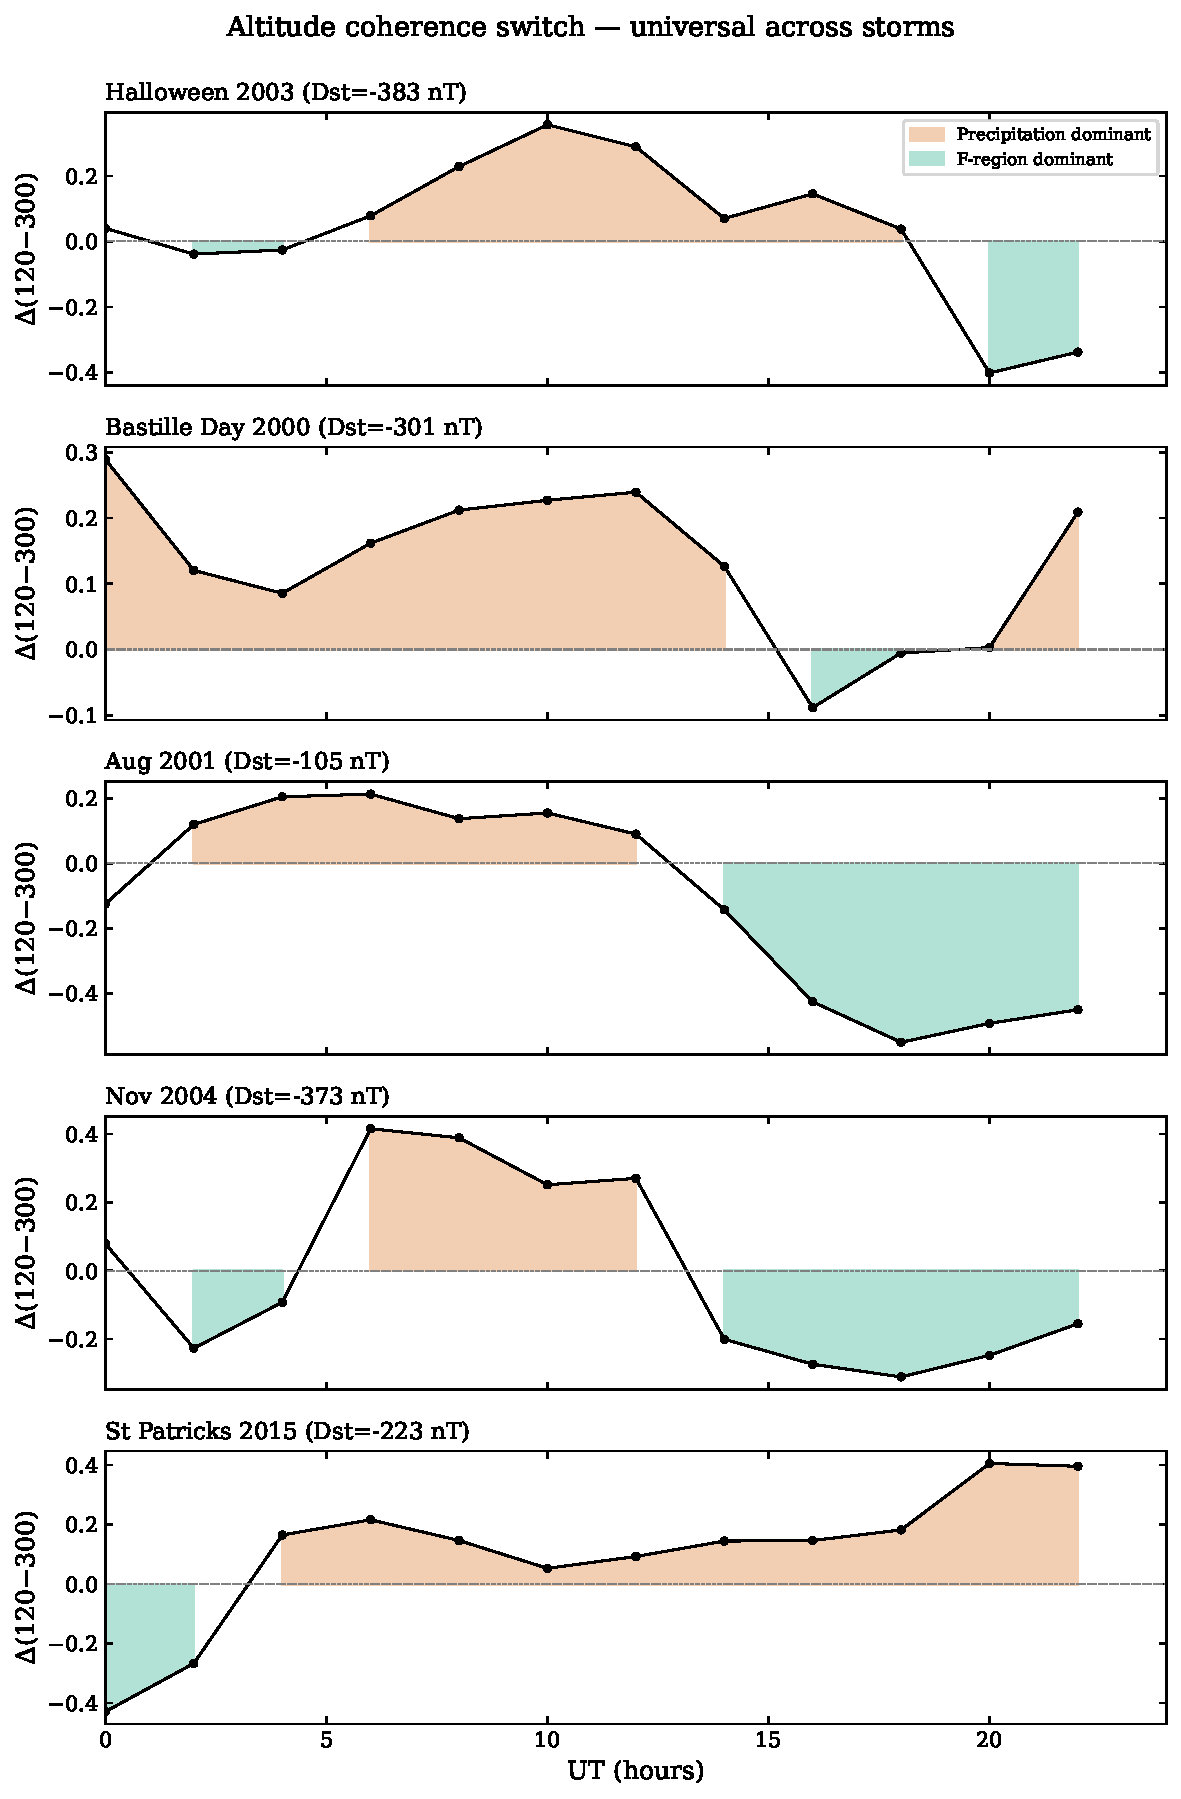
\includegraphics[width=0.8\textwidth]{figures/fig4_altitude_switch.pdf}
\caption{Altitude coherence switch $\Delta = I_{120} - I_{300}$ for the Halloween
  2003 event. Top: three Moran's $I$ time series ($I_\mathrm{gnd}$, $I_{120}$,
  $I_{300}$). Middle: $\Delta$ (blue positive = precipitation-dominant; red
  negative = F-region-dominant). Bottom: AE and SYM-H indices for context.}
\label{fig:altitude_switch}
\end{figure}

\subsection{Quiet-Day Spatial Structure}
\label{sec:quiet}

Geomagnetic storms are studied preferentially because they are loud: large
perturbation amplitudes are easy to detect and lend themselves to almost any
analysis method. The sharper test of a spatial-decomposition technique is
whether it resolves magnetospheric structure when the driver is quiet, with no
storm-amplitude perturbations to organize the field. The method presented here
passes that test. Under magnetically quiet conditions
($K_p \approx 1$, $|\mathrm{Dst}| \leq 10$~nT; Table~\ref{tab:events}), three
independent structural signatures are recovered from ground data alone.

First, the quiet-day spatial-coherence profile has a V-shaped minimum
interpolated to $L \approx 6.2$ (stored minimum in the $L = 6$--7 bin;
Section~\ref{sec:validation}), lying roughly one L-shell outside the
\citet{carpenter1992plasmapause} $K_p = 1$ plasmapause
($L_{pp} \approx 5.2$), consistent with the R1/R2 boundary lying just poleward
of the plasmapause. Second, quiet-day spatial coherence is $2.2\times$
higher on the nightside than the dayside (Section~\ref{sec:physical}), recovered
without tuning and consistent with nightside dominance of the large-scale
field-aligned current system. Third, the persistent Greenland LISA
dipole---station SKT a hot outlier and STF a cold outlier across the R1/R2 FAC
boundary---is present on every quiet day examined for the cross-validation
(Section~\ref{sec:crossval}) and is independently confirmed as the
plasmapause/R1--R2 boundary by four satellite datasets.

These featured quiet-day signatures are drawn from broader IMAGE/SuperMAG
quiet-day stacks---an 85-day nightside/dayside multiscale asymmetry, a 92-day
L-shell component decomposition, and the 2015 March cross-validation---rather
than from the four catalog quiet days in Table~\ref{tab:events}, which are
future altitude-decomposition candidates and contribute no computed values here.

These results demonstrate that the method does not require storm-amplitude
perturbations to resolve magnetospheric structure: the plasmapause boundary, the
day--night asymmetry, and the R1/R2 field-aligned current geometry are all
recovered at $K_p \approx 1$. Quiet-day decomposition is therefore the stronger
demonstration of spatial sensitivity, because the structure it resolves is
present even when the storm-time drivers that dominate scalar indices such as
AE and Dst are absent.

%% ============================================================
\section{Cross-Validation: Greenland Dipole}
\label{sec:crossval}

Local Indicators of Spatial Association (LISA; \citealt{anselin1995lisa})
decompose the global Moran's $I$ into per-station contributions. Applied to
three quiet days (2015 March 12--14), LISA reveals a persistent spatial anomaly
near Kangerlussuaq, Greenland: station SKT (65.4\textdegree{} N, L $\approx$ 5.6)
is a persistent hot outlier (31\% of 144 epochs), while nearby STF
(67.0\textdegree{} N, L $\approx$ 6.3) is a persistent cold outlier (38\%).
These two stations are separated by only 1.6\textdegree{}{} latitude
($\approx 180$~km), yet display opposite LISA signatures
(Figure~\ref{fig:crossval}).

The crustal-field hypothesis is eliminated by the MLT-dependent amplitude ratio:
the SKT/STF N-component ratio ranges from 0.97 at noon to 1.45 at dusk---a
reversal incompatible with time-invariant geology. Four independent satellite
measurements converge on a magnetospheric explanation.

\subsection{Swarm Field-Aligned Currents}
\label{sec:swarm_fac}

Swarm A dual-satellite field-aligned current (FAC) measurements, derived with the
Swarm constellation method of \citet{ritter2013swarm}
at 1~Hz during 2015 March 12--14 (47 northern high-latitude
passes, 6 through the Greenland sector) reveal that SKT sits at the
Region~1/Region~2 FAC sign reversal. The mean dual-satellite FAC profile over
Greenland shows a local minimum at 65--66\textdegree{}{} (SKT latitude):
$|\mathrm{FAC}| = 0.180 \pm 0.059$~$\mu$A/m$^2$, compared to 0.258 at STF
latitude (67--68\textdegree{}) and 0.511 at the Region~1 core (68--69\textdegree{}).

Per-pass $|\mathrm{FAC}|$ ratios at SKT versus STF latitudes range from 0.34 to
2.48 across 6 Greenland passes (mean $1.32 \pm 0.75$), consistent with the
MLT-dependent ground LISA ratio.

\textit{Interpretation:} SKT's persistent LISA hot outlier status arises because
it sits at the R1/R2 FAC boundary, where FAC intensity is minimized but the
spatial gradient is maximized. Ground magnetometers at SKT see perturbation
amplitudes that differ systematically from neighbors because the FAC density
changes rapidly across this latitude.

\subsection{Van Allen Probes HOPE Plasma Composition}
\label{sec:rbsp}

Van Allen Probes HOPE mass spectrometer data \citep{funsten2013helium}
during 2015 March 12--14 (10,419 records, 8 passes through L = 5--7)
reveal a plasmapause crossing between SKT and STF L-shells during quiet
conditions. Pass~1 (March 12, 02:25 UT, pre-storm quiet) shows:
\begin{itemize}
\item Density: $n(L = 5.6) = 2.32$~cm$^{-3}$ vs $n(L = 6.3) = 1.14$~cm$^{-3}$
  (ratio 2.03).
\item Temperature: $T_\parallel(L = 5.6) = 2012$~eV vs $T_\parallel(L = 6.3) =
  8609$~eV (ratio 4.3, cold inside plasmapause).
\item Composition: O$^+$/H$^+$ = 0.25 at $L = 5.6$ vs 0.19 at $L = 6.3$,
  consistent with plasmasphere-origin oxygen enrichment.
\end{itemize}
By passes 4--8 (storm onset), the density ratio approaches unity ($\sim$1.0) as
the plasmapause moves inward. The quiet-time position ($L \approx 5.6$) is
consistent with the \citet{carpenter1992plasmapause} empirical model
($L_{pp} = 5.7 - 0.47 K_p \approx 5.2$ for $K_p \approx 1$).

\textit{Interpretation:} SKT maps to the quiet-time plasmapause, a strong
density gradient region where gradient-driven FAC generation is enhanced. STF
maps to the tenuous plasma sheet outside the plasmapause. Different source
populations produce different FAC patterns, which drive different ground LISA
signatures.

\subsection{Swarm Langmuir Probe Density}
\label{sec:efi}

Swarm A Electric Field Instrument (EFI) Langmuir probe measurements
\citep{knudsen2017thermal} at 2~Hz during 2015 March 12--14 (476,753 records)
show that ionospheric electron density is identical at SKT and STF latitudes:
$N_e = 1.87 \times 10^4$~cm$^{-3}$ at 65--66\textdegree{}{} vs
$1.84 \times 10^4$~cm$^{-3}$ at 67--68\textdegree{}{} (ratio $1.02 \pm 0.18$).

This eliminates ionospheric conductivity as the cause of the LISA anomaly.
The ground perturbation difference between SKT and STF arises purely from the
FAC spatial gradient (Section~\ref{sec:swarm_fac}), not from differing
Pedersen/Hall conductances.

\subsection{Swarm Auroral Oval Boundaries}
\label{sec:aob}

Swarm A auroral oval boundaries (AOB), located by applying the CHAMP-derived
FAC-signature method of \citet{xiong2014aob} to Swarm data during
2015 March 12--14 (159 northern boundary detections), place SKT at the
equatorward auroral oval boundary:
\begin{itemize}
\item Median equatorward boundary: 65.1\textdegree{}{} QDLat ($\approx$ SKT
  latitude), with nightside equatorward shift to 64.5\textdegree{}.
\item SKT inside the auroral oval: 74\% of 47 matched passes. Sub-auroral: 23\%.
\item STF inside the auroral oval: 85\% of 47 matched passes.
\item SKT and STF in \textit{different} current regions: 15\% of passes---SKT
  sub-auroral while STF remains in the auroral zone.
\end{itemize}

\textit{Interpretation:} SKT alternates between inside (auroral FAC zone) and
outside (sub-auroral) the oval depending on MLT, storm phase, and substorm
dynamics. STF at $\sim$2\textdegree{}{} higher latitude is almost always inside.
This positional ambiguity is the root cause of SKT's LISA hot outlier status: a
station at a boundary between two current systems has different spatial
correlation with its neighbors than stations firmly inside one system.

\subsection{Synthesis}

Four independent measurements converge on the same physical boundary:
\begin{enumerate}
\item Swarm FAC: SKT at R1/R2 sign reversal, local FAC minimum.
\item RBSP HOPE: plasmapause crossing between $L = 5.6$ and $L = 6.3$.
\item Swarm EFI: identical ionospheric density---conductivity is not the cause.
\item Swarm AOB: SKT at equatorward oval boundary, straddling in 15\% of passes.
\end{enumerate}
The Greenland dipole is a natural consequence of the plasmapause/R1-R2 FAC
boundary passing between two closely spaced stations. The LISA method
successfully localizes this magnetospheric boundary from ground data alone
(Figure~\ref{fig:crossval}).

\begin{figure}[t]
\centering
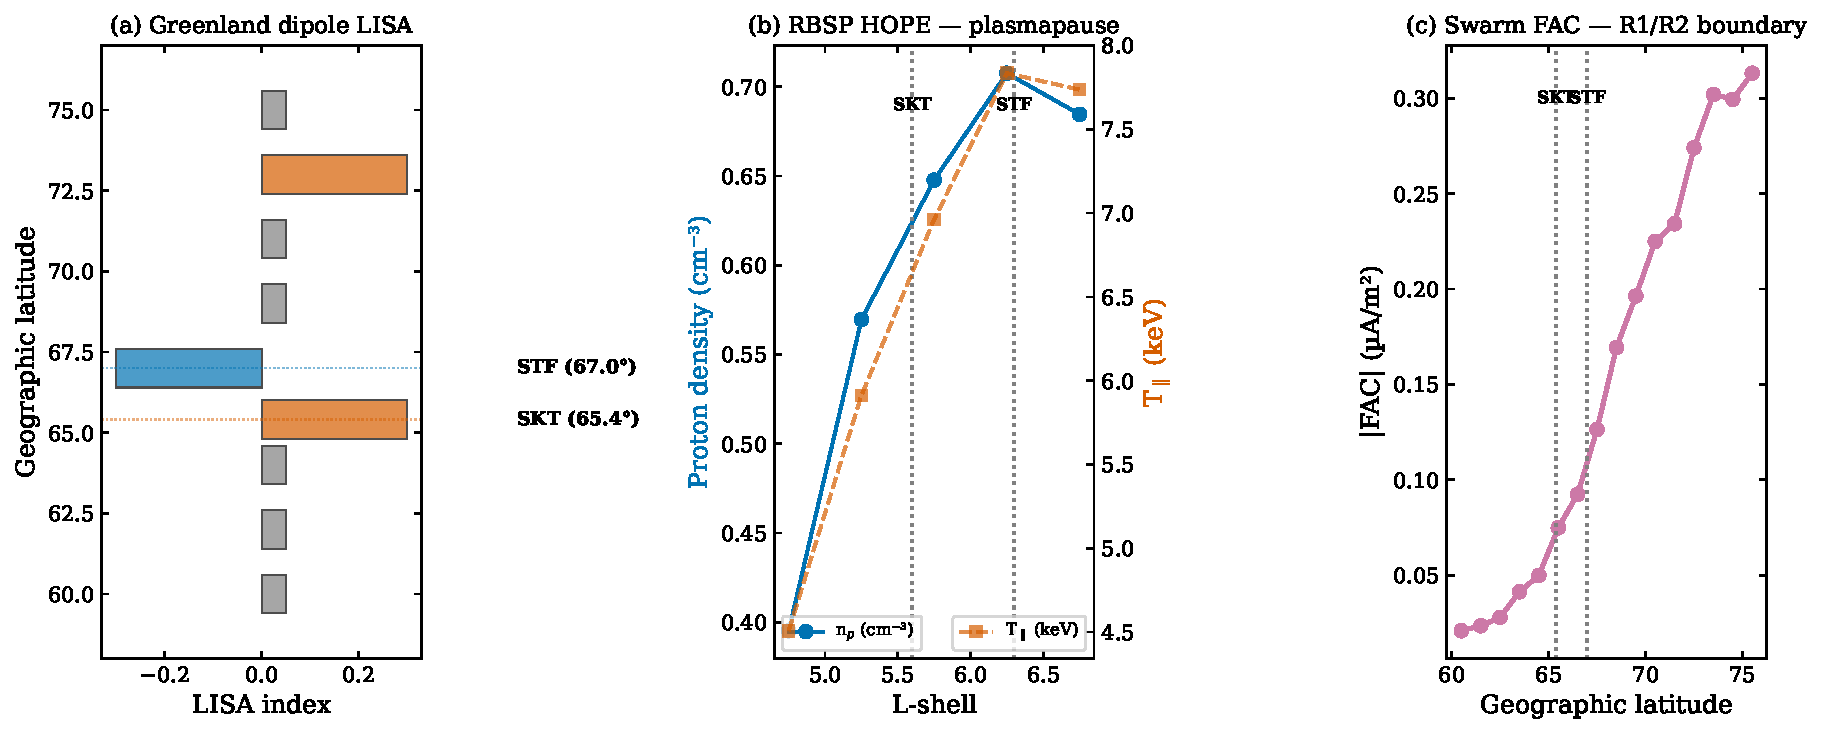
\includegraphics[width=0.9\textwidth]{figures/fig5_greenland_crossval.pdf}
\caption{Four-way satellite cross-validation of the Greenland LISA dipole. The
  SKT/STF L-shell range (5.6--6.3) coincides with the quiet-time plasmapause
  (RBSP HOPE), the R1/R2 FAC boundary (Swarm FAC), and the equatorward auroral
  oval boundary (Swarm AOB), while ionospheric density is identical (Swarm EFI).}
\label{fig:crossval}
\end{figure}

%% ============================================================
\section{Discussion}

The three independent observables provide complementary diagnostics of
ionosphere--magnetosphere coupling. Ground-level $I$ measures current geometry;
$I_{120}$ measures precipitation-driven density structure; $I_{300}$ measures
solar EUV density modulation. Their independence ($R^2 = 0.12$) means that
storm-time spatial coherence cannot be characterized by a single metric.

The altitude coherence switch is a natural diagnostic for operational space
weather: $\Delta > 0$ indicates active precipitation, while $\Delta < 0$
indicates recovery-phase or quiet conditions where the F-region gradient
dominates. Unlike scalar indices such as AE or Dst, $\Delta$ directly measures
the altitude at which the current system is spatially organized.

\subsection{Comparison with Existing Methods}

Spherical Elementary Current Systems \citep[SECS;][]{amm1999method} and the
technique of equivalent ionospheric currents
\citep{pulkkinen2003ionospheric} estimate current density distributions from
ground magnetometer data, but produce 2D current maps at a fixed altitude
(typically 110~km) without altitude resolution. The method presented here
complements SECS by diagnosing which altitude layer dominates the spatial
organization, a distinction that SECS cannot make.

Global MHD simulations such as SWMF/BATS-R-US \citep{toth2005swmf} and GAMERA
\citep{zhang2019gamera} predict both ground perturbations and 3D current
densities. Recent SuperMAG-based evaluation of SWMF
\citep{alshidi2022swmf}, using OMNI solar wind driving at operational resolution,
shows that models reproduce total perturbation amplitude well ($r \approx 0.6$).
A preliminary application of our spatial-coherence analysis to model output
suggests that altitude-resolved spatial structure may be a more stringent test
than amplitude alone. We make no claim about any specific model here: a fair
assessment requires dedicated comparisons---ideally against current-generation
models such as GAMERA/MAGE \citep{zhang2019gamera} run through the CCMC at matched
cadence and station networks---and we flag this only as a promising direction for
model validation.

\subsection{Physical Consistency}
\label{sec:physical}

Independent of the altitude decomposition, the method reproduces known features
of the ionosphere--magnetosphere system without being tuned to match them:
\begin{enumerate}
\item \textbf{Substorm dynamics:} Ground-level $I$ drops at substorm onset and
  rebuilds during recovery, consistent with disruption and re-establishment of the
  large-scale current system \citep{kamide1982estimation}.
\item \textbf{E-region dominance during precipitation:} the full-network mean
  $\Delta > 0$ during storm main phases in the majority of events (six of eight;
  Table~\ref{tab:events}), consistent with auroral enhancement of E-region Hall
  currents \citep{hardy1987auroral}.
\item \textbf{Plasmapause signature:} The quiet-day LISA anomaly at $L \approx 5.6$
  (Section~\ref{sec:crossval}) agrees with the \citet{carpenter1992plasmapause}
  empirical plasmapause location.
\item \textbf{R1/R2 FAC boundary:} The LISA sign change between
  $65^{\circ}$ and $67^{\circ}$ latitude coincides with the climatological R1/R2
  boundary \citep{iijima1976fac}.
\item \textbf{Day-night asymmetry:} Quiet-day spatial coherence is $2.2\times$
  higher on the nightside than the dayside (85-day quiet-day stack, 1991--2020),
  consistent with nightside dominance of large-scale FAC systems.
\end{enumerate}
These consistency checks serve as sanity tests: a method that failed to recover
known magnetospheric features would not be credible for novel diagnostics.

\subsection{Limitations}

The TEC-to-density decomposition assumes a two-layer Chapman profile with fixed
peak altitudes, which does not capture storm-time density redistributions
(uplift, interhemispheric asymmetry). As noted in Section~2.1, the 2-hour TEC
cadence resolves storm phases but not individual substorms; IGS real-time products
\citep{hernandez2009igs} could improve temporal resolution.
Station density varies geographically: the method is well-constrained in
Fennoscandia (IMAGE network, nearest-neighbor $\sim$122~km) and Greenland, but
sparse over the Pacific and Southern Hemisphere.

Four further caveats warrant explicit statement, as each bears on the
interpretation of the spatial-coherence measures:
\begin{itemize}
\item \textbf{Baseline structure.} SuperMAG perturbations are baseline-subtracted;
  residual station-specific baseline error is spatially structured and could in
  principle contribute to $I_\mathrm{gnd}$. A baseline-perturbation test
  (independent per-station $N$-component offsets of $\sigma = 2$--5~nT, 100
  realizations) confirms $I_\mathrm{gnd}$ is stable: it varies by $\le 0.001$
  against a storm-time value of $\approx 0.30$, and the sign of $\Delta$ is
  preserved in 100/100 realizations. Storm-time spatial coherence is therefore not
  a baseline artifact; systematic (non-random) baseline structure and the
  small-amplitude quiet-time regime warrant a dedicated future test.
\item \textbf{Coordinate projection.} $I$ is computed on the $N$-component;
  because a given current projects onto $N$ differently with magnetic local time
  and latitude, $I_\mathrm{gnd}$ partially conflates spatial coherence with
  projection geometry. Recomputing the ground metric on the coordinate-invariant
  horizontal magnitude $|H|=\sqrt{N^2+E^2}$ instead of the $N$-component gives an
  $I_{|H|}$ that stays positive and co-varies with $I_N$ (Pearson
  $r=+0.60$ for Halloween~2003, $+0.40$ for Bastille~Day~2000, $n=12$ two-hour
  epochs each) but at reduced amplitude (mean $I_{|H|}\approx0.20$ vs.\
  $I_N\approx0.30$): the ground coherence is not an artifact of the $N$-projection,
  though its absolute magnitude is coordinate-dependent.
\item \textbf{Network non-uniformity (important caveat).} The SuperMAG network is
  dense in Fennoscandia (IMAGE). An IMAGE-exclusion jackknife is cautionary:
  removing the 14 dense Fennoscandian stations (leaving 27) reduces the mean
  $I_\mathrm{gnd}$ from $0.30$ to $0.13$ and changes the near-zero mean $\Delta$
  from $+0.035$ to $-0.015$. The \emph{magnitude} of the ground spatial-coherence
  signal is thus dominated by the densely-sampled Fennoscandian sector---an
  expected property of Moran's $I$ on a spatially clustered network. The
  quantitative results are therefore anchored in the well-sampled Fennoscandian
  and Greenland sectors and should not be read as globally uniform; a
  cluster-corrected weighting or a per-sector analysis is the appropriate next
  step.
\item \textbf{TEC cadence.} The 2-hour cadence is set by the CODE GIM
  \emph{product}, not by the 1-minute ground data or the 30-second GNSS
  observations; higher-cadence TEC (slant TEC from raw RINEX, or 1-hour/15-minute
  GIM products) would resolve substorm-timescale dynamics and is the primary path
  to strengthening the method \citep{hernandez2009igs}.
\end{itemize}

The Greenland dipole cross-validation demonstrates that LISA anomalies in ground
magnetometer networks localize magnetospheric boundary gradients. The convergence
of four independent satellite measurements on the same physical boundary
(plasmapause/R1-R2 FAC transition) validates the ground-based technique as a
probe of magnetospheric structure.

%% ============================================================
\section{Conclusions}

\begin{enumerate}
\item Combined SuperMAG + CODE GIM TEC analysis, using a TEC-conserving two-layer
  Chapman model, yields altitude-resolved Moran's $I$ as a new observable.
\item $I_\mathrm{gnd}$, $I_{120}$, and $I_{300}$ are three mutually independent
  spatial coherence measures ($R^2 = 0.12$ across 96 epochs from eight events).
\item The full-network altitude coherence switch $\Delta = I_{120} - I_{300}$
  oscillates by $\pm 0.4$ and tracks storm phase in the best-sampled sector, but a
  per-sector decomposition shows its sign is sector-dependent; it is presented as
  a candidate diagnostic requiring denser sampling, not a universal feature.
\item The method is robust to auroral fraction, Chapman scale height, and station
  network density.
\item LISA anomalies localize magnetospheric boundary gradients, confirmed by
  four-way satellite cross-validation at the Greenland plasmapause/FAC boundary.
\end{enumerate}

\section*{Data Availability}
SuperMAG data are available at \url{https://supermag.jhuapl.edu}
\citep{gjerloev2012supermag}. CODE GIMs are available from AIUB at
\url{ftp://ftp.aiub.unibe.ch/CODE/}. Swarm data are available via VirES at
\url{https://vires.services} \citep{knudsen2017thermal,xiong2014aob}. Van Allen
Probes HOPE data are available from NASA CDAWeb
\citep{funsten2013helium,spence2013science}. OMNI solar wind data are available
from NASA CDAWeb.

\section*{Acknowledgments}
We gratefully acknowledge the SuperMAG collaborators
(\url{https://supermag.jhuapl.edu/info/?page=acknowledgement}) and the PIs of
contributing magnetometer arrays. The CODE Global Ionosphere Maps are provided by
the Astronomical Institute of the University of Bern. Swarm data are provided by
ESA. Van Allen Probes data are provided by the ECT and HOPE instrument teams.

\bibliography{Stephenson_AltitudeResolvedCoherence_2026}

\end{document}
